\section*{CHƯƠNG 4: KẾT QUẢ THỰC HIỆN}
\addcontentsline{toc}{section}{\numberline {} CHƯƠNG 4: KẾT QUẢ THỰC HIỆN}
\setcounter{section}{4}
\setcounter{figure}{0}
\setcounter{subsection}{0}
\subsection{KẾT QUẢ THI CÔNG PHẦN CỨNG}
\begin{figure}[H]
	\centering
	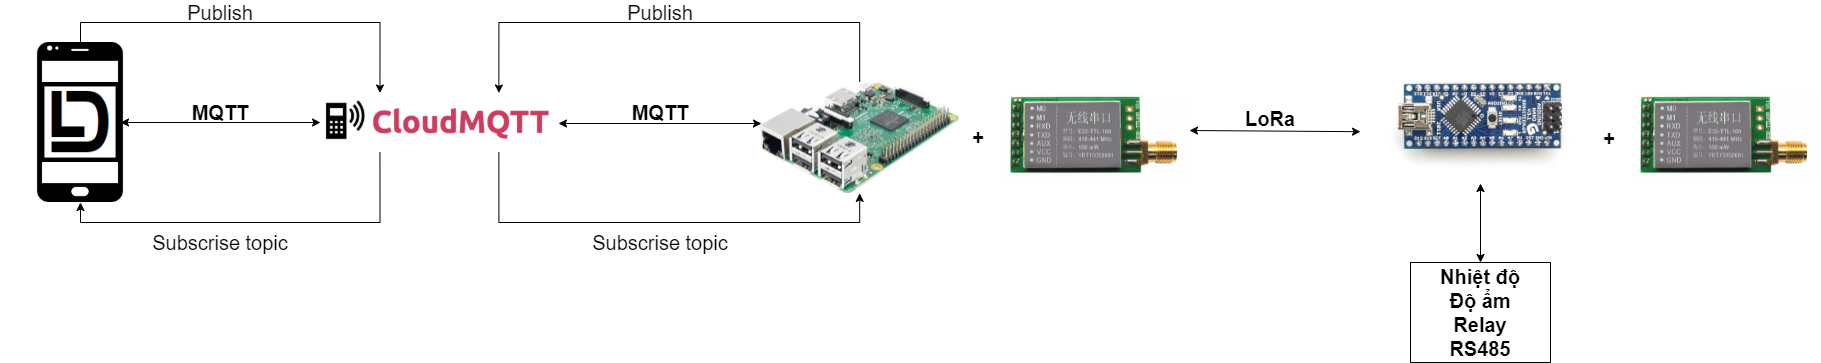
\includegraphics[scale=0.2]{Chapter 4/image chapter 4/figure.png}
	\caption[Sơ đồ các giao tiếp phần cứng]{Sơ đồ các giao tiếp phần cứng}
	\label{hinh41}
\end{figure}
\begin{figure}[H]
	\centering
	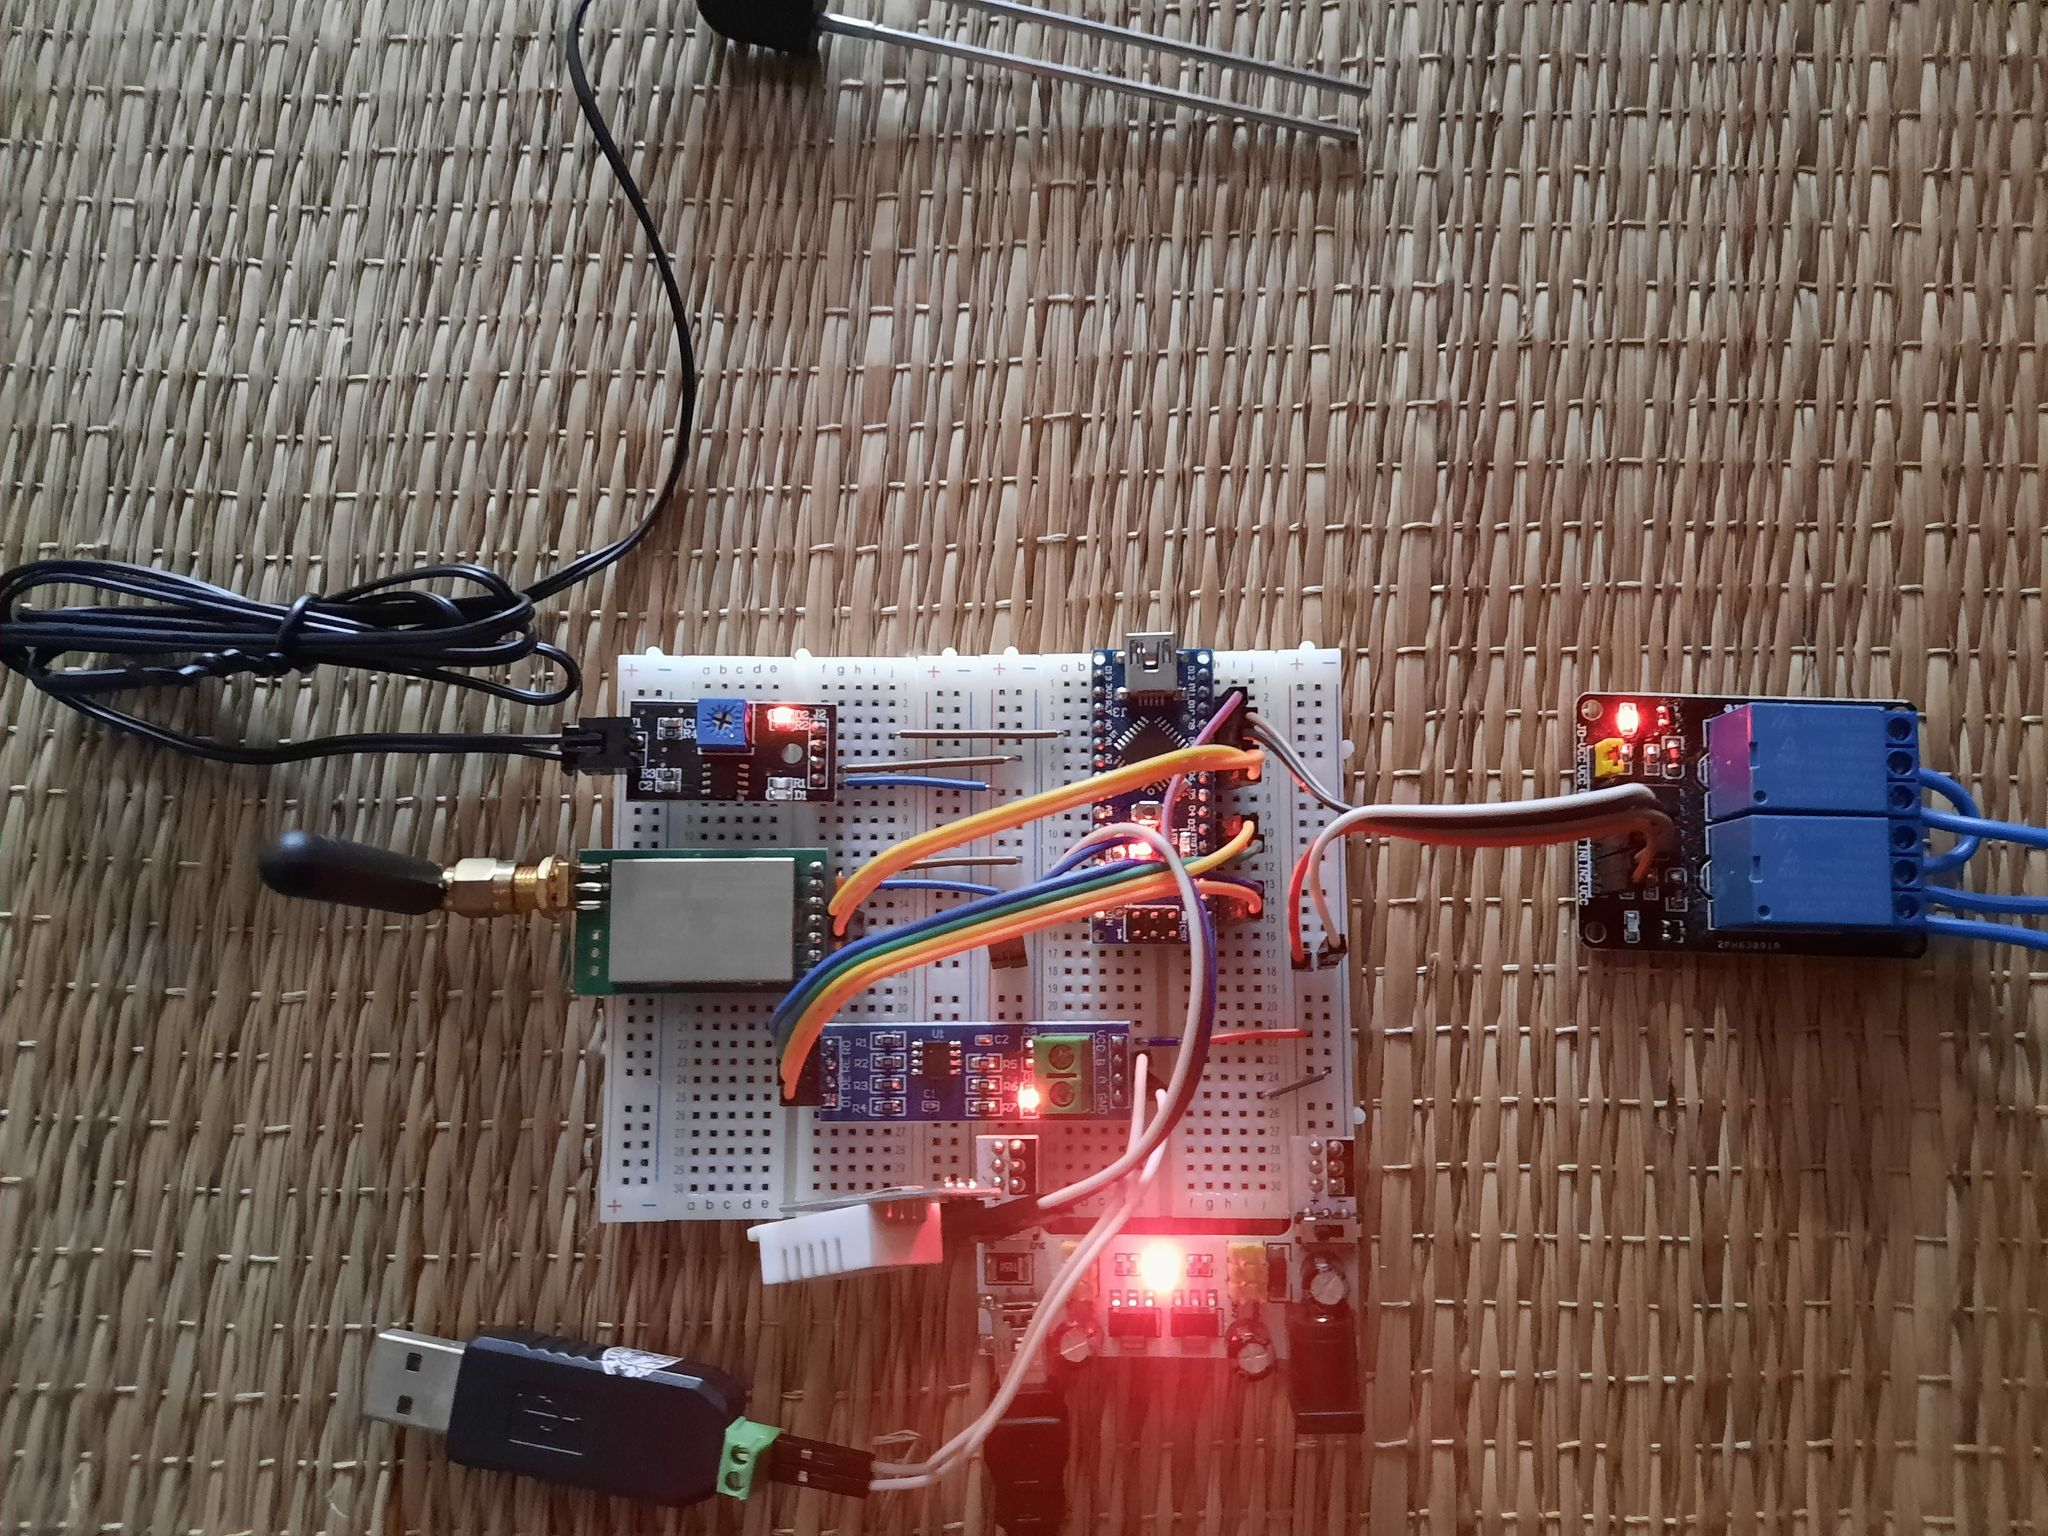
\includegraphics[scale=0.2]{Chapter 4/image chapter 4/phancung.jpg}
	\caption[Phần cứng end-Node trong thực tế]{Phần cứng end-Node trong thực tế}
	\label{hinh42}
\end{figure}
\subsection{KIỂM TRA ĐỘ CHÍNH XÁC THÔNG SỐ NHIỆT ĐỘ \& ĐỘ ẨM}
\subsection{KIỂM TRA HOẠT ĐỘNG CỦA MODULE 2 RELAY}